\section{Utilizzo di Butterfly}\label{utilizzo}

\subsection{Gestore Personale}

Il Gestore Personale è la componente principale di \progetto\ e si può suddividere in due sotto-componenti principali:

\begin{itemize}
    \item Interfaccia utente a sua volta divisa in
    \begin{itemize}
    	\item Interfaccia amministratore
    	\item Interfaccia Utente (senza permessi amministratore)
    \end{itemize}
    \item Message processor, che contiene la logica di business di \progetto
\end{itemize}

Il secondo non è di pertinenza di questo manuale (ma del \MSd), in quanto l'utente non lo utilizza direttamente, per cui verrà solamente discusso l'utilizzo del sistema tramite l'interfaccia utente.

\subsubsection{Interfaccia Utente}
Le seguenti opzioni del Gestore Personale sono accessibili da ogni tipo utente, perciò anche da quelli coi privilegi di amministratore.

\paragraph{Accesso}
È possibile effettuare l'accesso all'interno del sistema tramite il link del container sul quale è in esecuzione, specificato nella configurazione effettuata precedentemente.
Per effettuare correttamente l'accesso è necessario l'inserimento del proprio ID Telegram o Email con il quale si è iscritti nel sistema.
\begin{figure}[H]
	\centering
	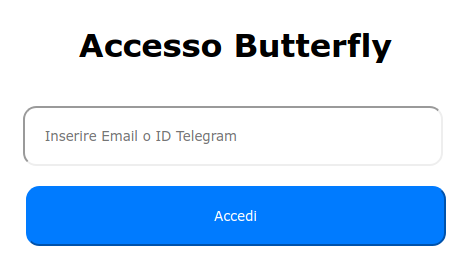
\includegraphics[width=9cm]{img/accesso_1.png}
	\caption{Form di accesso al sistema}
\end{figure}
In caso l'identificativo inserito non fosse valido, e non corrispondesse quindi a un match nel database, verrà mostrato all'utente un messaggio di errore.
\begin{figure}[H]
	\centering
	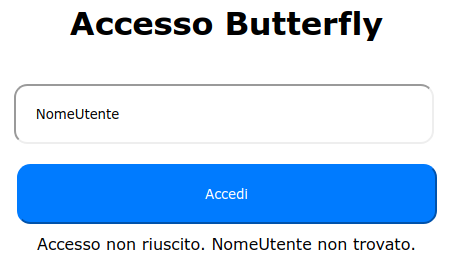
\includegraphics[width=9cm]{img/accesso_2.png}
	\caption{Messaggio di errore durante accesso al sistema}
\end{figure}

Nel caso in cui un utente cerchi di accedere ad una sezione, ma senza aver effettuato l'accesso, questo verrà rimandato alla pagina di accesso.\par
Se un utente iscritto correttamente nel sistema ha registrato precedentemente sia indirizzo Email che ID Telegram, allora può accedere utilizzando indipendentemente il primo o il secondo.

\paragraph{Pannello di controllo}
Dopo aver effettuato l'accesso al sistema, si viene rimandati alla pagina relativa al Pannello di controllo che contiene i comandi principali per la navigazione del sito e le operazioni che un utente può eseguire.
Le sezioni a cui si può navigare dal Pannello di controllo sono:
\begin{itemize}
	\item Modifica dei propri dati
	\item Modifica delle proprie preferenze
\end{itemize}

\paragraph{Modifica preferenze}\label{preferenze}
La modifica delle preferenze è possibile solamente per utenti già iscritti ed autenticati nel sistema.
È raggiungibile tramite il Pannello di Controllo sotto la voce ``Modifica le tue preferenze''.
In questa sezione si possono trovare le principali impostazioni del sistema dal punto di vista dell'utente finale:
\begin{itemize}
	\item Lista dei progetti a cui si è iscritti
	\item Modifica della priorità assegnata ad un progetto
	\item Lista dei Topic (formati dall'insieme di label e keyword) disponibili e iscrizione o disiscrizione da questi, che vengono mostrati dinamicamente in base ai progetti a cui si è iscritti
	\item Inserimento dei giorni di indisponibilità
	\item Impostare su quale delle due piattaforme di messaggistica (Email o Telegram) ricevere le notifiche
\end{itemize}
Le ``label'' non sono modificabili in quanto vengono aggiornate solamente da una componente del Gestore Personale che le memorizza quando avvengono \gloss{update} alle issue relative ai progetti.
Le ``keyword'' invece, sono formate da una lista di parole che possono essere contenute nei messaggi di push di GitLab e di cui si è interessati a ricevere notifiche.
\begin{figure}[H]
	\centering
	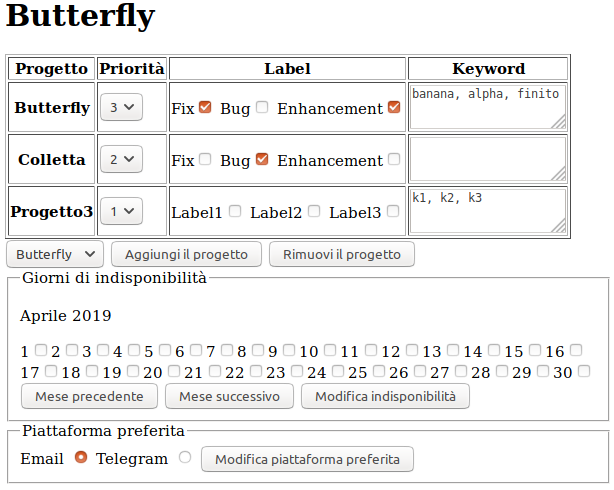
\includegraphics[width=12cm]{img/preferenze_1.png}
	\caption{Interfaccia modifica preferenze}
\end{figure}

\paragraph{Modifica dei propri dati}
La modifica dei propri dati è possibile attraverso la sezione ``Modifica i tuoi dati'' accessibile dal Pannello di Controllo.
Qui un utente può modificare i dati inseriti dall'amministratore in fase di registrazione.
\begin{figure}[H]
	\centering
	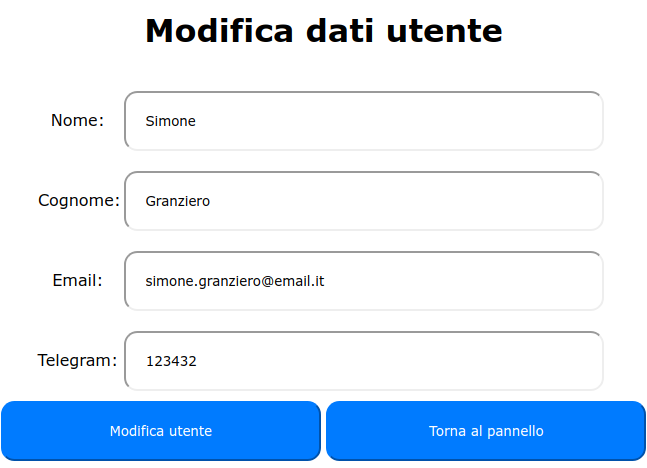
\includegraphics[width=\textwidth]{img/modifica_1.png}
	\caption{Modifica dei dati di un utente}
\end{figure}
Nel caso questi fossero già associati ad una persona iscritta a \progetto, verrà visualizzato un messaggio di errore.

\paragraph{Uscita dal sistema}
Per effettuare il logout dal sistema, cliccare sul bottone ``Logout'' presente in alto a destra di ciascuna pagina.

\subsubsection{Interfaccia amministratore}
All'interno dell'applicazione \progetto, gli utenti coi permesso di amministratore potranno eseguire le stesse azioni di un utente normale e in più gestire l'insieme degli utenti iscritti al sistema. Per un utente amministratore non esiste un particolare sistema di accesso, infatti accede come ogni altro utente.

\paragraph{Pannello di controllo}
Dopo aver effettuato l'accesso al sistema, si viene rimandati alla pagina relativa al Pannello di controllo che contiene i comandi principali per la navigazione del sito e le operazioni che un utente può eseguire.
Le sezioni a cui si può navigare dal Pannello di controllo sono:
\begin{itemize}
    \item Inserimento di un nuovo utente
    \item Rimozione di un utente
    \item Modifica dei propri dati
    \item Modifica delle proprie preferenze
\end{itemize}
\begin{figure}[H]
    \centering
    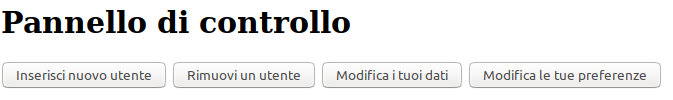
\includegraphics[width=14cm]{img/pannello_1.png}
    \caption{Interfaccia modifica preferenze}
\end{figure}

\paragraph{Iscrizione a Butterfly}\label{Iscrizione}
L'iscrizione di un nuovo utente al sistema \progetto\ è permessa solamente all'utente amministratore.
La sezione di inserimento di un nuovo utente è raggiungibile dal Pannello di controllo e prevede l'inserimento dei seguenti dati:
\begin{itemize}
	\item Nome
	\item Cognome
	\item Email
	\item Telegram
\end{itemize}
\begin{figure}[H]
	\centering
	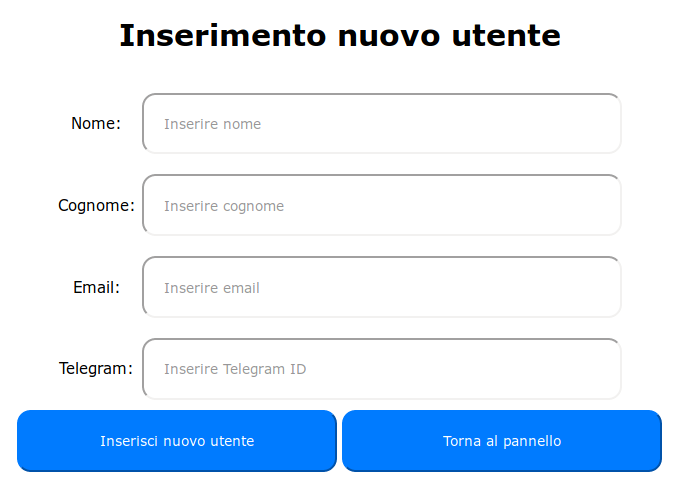
\includegraphics[width=\textwidth]{img/inserimento_1.png}
	\caption{Interfaccia inserimento nuovo utente}
\end{figure}
Nel caso questi fossero già associati ad un utente iscritto a \progetto\ verrà visualizzato un messaggio di errore.

È necessario inserire almeno un campo a scelta tra Email e Telegram.
Nel caso questi fossero già associati ad un utente iscritto a \progetto\ verrà visualizzato un messaggio di errore.

\paragraph{Rimozione di un utente dal sistema}\label{Rimozione}
Viene data la possibilità di rimuovere un utente dal sistema solamente all'amministratore.
La rimozione è possibile attraverso la sezione ``Rimuovi un utente'' accessibile dal Pannello di Controllo.
\begin{figure}[H]
	\centering
	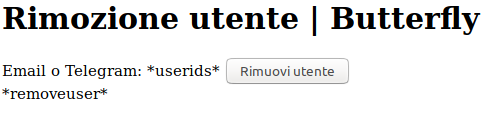
\includegraphics[width=12cm]{img/rimozione_1.png}
	\caption{Interfaccia rimozione di un utente}
\end{figure}

\paragraph{Visualizzazione lista di utenti}
Un utente amministratore ha la possibilità di vedere la lista di tutti gli utenti iscritti al sistema e i relativi progetti a cui sono interessati.
La visualizzazione avviene attraverso la sezione ``Lista utenti'' accessibile dal Pannello di Controllo.
\begin{figure}[H]
	\centering
	\caption{Interfaccia lista degli utenti}
\end{figure}

\subsection{API Rest}\label{APIRest}
\newcommand{\homeUrl}{home\_url}

Per la gestione delle risorse di \progetto\ abbiamo utilizzato lo standard architetturale delle API Rest.
Nelle sezioni successive viene descritto come interagire con le API fornite dal sistema.
Il \gloss{root path} sottinteso sarà sempre \texttt{\homeUrl/api/v1/}.
Ad esempio, per effettuare la GET dell'user \texttt{@user1}, l'indirizzo sarà:
\begin{center}
    \texttt{GET \homeUrl/api/v1/user/@user1}
\end{center}

\subsubsection{User}

\texttt{User} è la risorsa utente.
È possibile visualizzare, aggiungere, modificare o rimuovere gli utenti tramite una semplice
richiesta HTTP.

\paragraph{Visualizzazione}
È possibile visualizzare i dati di un utente tramite la richiesta
    \begin{center}
        \texttt{GET  /user/<id>}
    \end{center}

\paragraph{Inserimento}
È possibile inserire un nuovo utente tramite la richiesta:
    \begin{center}
        \texttt{POST /user}
    \end{center}

È inoltre possibile dare i seguenti campi di tipo stringa alla richiesta, per aggiungere in fase di creazione i dati:
\begin{itemize}[noitemsep]
    \item \texttt{name}
    \item \texttt{surname}
    \item \texttt{telegram}
    \item \texttt{email}
\end{itemize}
Almeno uno tra i campi \texttt{email} e \texttt{telegram} vanno fornite insieme al \gloss{payload}.

\paragraph{Modifica}

È possibile modificare un utente tramite la richiesta
\begin{center}
    \texttt{PUT /user/<id>}
\end{center}

È possibile dare i seguenti campi di tipo stringa alla richiesta, per aggiungere in fase di creazione i dati:
\begin{itemize}[noitemsep]
    \item \texttt{name}
    \item \texttt{surname}
    \item \texttt{telegram}
    \item \texttt{email}
\end{itemize}


\paragraph{Rimozione}

È possibile rimuovere un utente dal sistema \progetto\ con la richiesta
\begin{center}
    \texttt{DELETE /user/<id>}
\end{center}

Se il campo \texttt{<id>} corrisponde a un ID presente nel sistema, esso verrà rimosso.


\paragraph{Riepilogo}

\begin{table}[H]
    \begin{paddedtablex}[1.3]{\textwidth}{cYY}
        \thead{Metodo HTTP} & \thead{URI} & \thead{Action}\\\toprule
        \texttt{GET} & \texttt{/user/<id>} & Restituisce un payload in JSON dell'utente che corrisponde a \texttt{<id>}\\
        \texttt{POST} & \texttt{/user} & Inserisce un nuovo utente. È necessario fornire uno tra i campi telegram o email\\
        \texttt{PUT} & \texttt{/user/<id>} & Modifica l'utente corrispondente a \texttt{<id>} con i campi passati nella richiesta\\
        \texttt{DELETE} & \texttt{/user/<id>} & Elimina l'utente corrispondente a \texttt{<id>} dal sistema\\
        \bottomrule
    \end{paddedtablex}
    \caption{Riepilogo delle Rest API per la risorsa User}
\end{table}


\subsubsection{Project}
Project è la risorsa relativa ai progetti. È possibile visualizzare, aggiungere, modificare o rimuovere i progetti di un utente tramite una semplice richiesta HTTP.

\paragraph{Visualizzazione}
È possibile visualizzare i progetti tramite la richiesta
    \begin{center}
        \texttt{GET /project/<id>}
    \end{center}
Se il campo \texttt{<id>} corrisponde a un progetto, verranno mostrati i dati relativi a tale progetto.

% I tipi di progetto disponibili sono:
% \begin{itemize}[noitemsep]
%     \item \texttt{progetto}
%     \item \texttt{disponibilità}
%     \item \texttt{piattaforma}
% \end{itemize}

\paragraph{Inserimento}
È possibile inserire un nuovo progetto tramite la richiesta
    \begin{center}
        \texttt{POST /project}
    \end{center}

È possibile fornire dei campi di tipo stringa alla richiesta, in base al tipo della risorsa, per aggiungere dati in fase di creazione.
I campi sono:
\begin{itemize}[noitemsep]
    \item \texttt{url}
    \item \texttt{app}
    \item \texttt{name}
    \item \texttt{topics}, una lista
\end{itemize}


\paragraph{Modifica}

È possibile modificare un progetto tramite la richiesta
\begin{center}
    \texttt{PUT /project/<id>}
\end{center}


È possibile fornire dei campi di tipo stringa alla richiesta, in base al tipo della risorsa, per aggiungere dati in fase di creazione.
I campi sono:
\begin{itemize}[noitemsep]
    \item \texttt{url}
    \item \texttt{app}
    \item \texttt{name}
    \item \texttt{topics}, una lista
\end{itemize}


\paragraph{Rimozione}

È possibile rimuovere un progetto dal sistema Butterfly con la richiesta
\begin{center}
    \texttt{DELETE /project/<id>}
\end{center}

Se il campo \texttt{<id>} corrisponde a un progetto, essa verrà rimossa dal sistema.

\paragraph{Riepilogo}

\begin{table}[H]
    \begin{paddedtablex}[1.3]{\textwidth}{cYY}
        \thead{Metodo HTTP} & \thead{URI} & \thead{Action}\\\toprule
        \texttt{GET} & \texttt{/project/<id>} & Restituisce un payload in JSON del progetto corrispondente a \texttt{<id>}\\
        \texttt{POST} & \texttt{/project} & Inserisce un nuovo progetto \\
        \texttt{PUT} & \texttt{/project/<id>} & Modifica il progetto corrispondente a \texttt{<id>} con i campi passati nel payload \\
        \texttt{DELETE} & \texttt{/project/<id>} & Elimina il progetto corrispondente a \texttt{<id>} dal sistema \\
        \bottomrule
    \end{paddedtablex}
    \caption{Riepilogo delle Rest API per la risorsa project}
\end{table}

\newpage

\subsection{Piattaforma di messaggistica}

\subsubsection{Email}

Per ricevere i messaggi di Butterfly tramite Email, è sufficiente fornire tramite l'interfaccia del Gestore Personale l'Email sulla quale si vuole ricevere la notifica.

\begin{figure}[H]
	\centering
	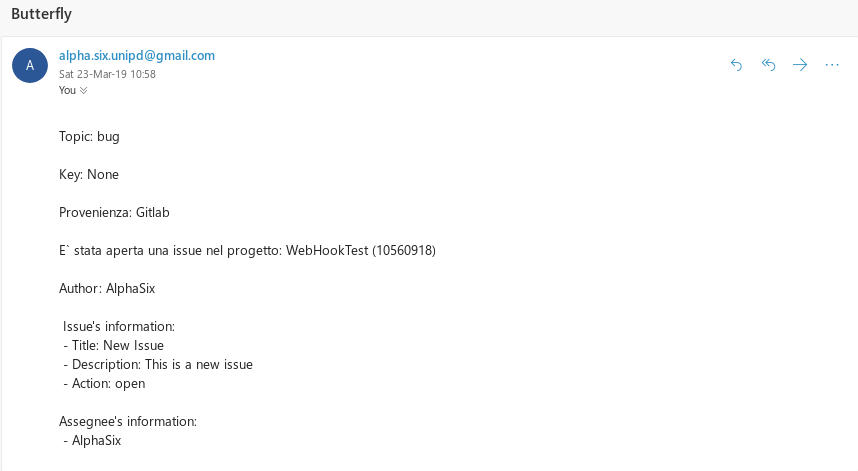
\includegraphics[width=\textwidth]{img/notifica_email_1.png}
	\caption{Formato dell' Email ricevuta da un utente finale}
\end{figure}

\subsubsection{Telegram}

Per ricevere le notifiche via Telegram, è necessario fare un passaggio addizionale: va fornita l'autorizzazione al bot per poter inviare messaggi agli utenti.
Il bot è raggiungibile al seguente link:
\begin{center}
    \url{http://t.me/ButterflyBot}
\end{center}

Dare il comando \texttt{/start} per dare l'autorizzazione di inoltro dei messaggi al bot.
È necessario inoltre aggiungere tramite l'interfaccia del Gestore Personale il proprio account Telegram.
In qualsiasi momento sarà possibile bloccare il bot in caso non si vogliano più ricevere messaggi relativi a Butterfly su Telegram, tramite le funzionalità dell'applicazione.
\begin{figure}[H]
	\centering
	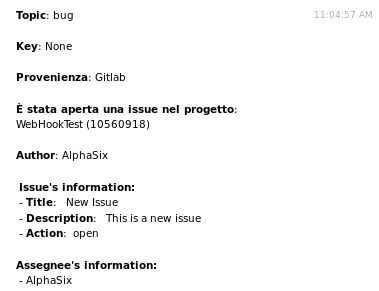
\includegraphics[width=9cm]{img/notifica_telegram_1.png}
	\caption{Formato del messaggio Telegram ricevuto da un utente finale}
\end{figure}
Nel caso in cui si volesse utilizzare un altro bot, i passaggi da seguire possono essere trovati sulla pagina apposita della documentazione di Telegram\footnote{\url{https://core.telegram.org/bots}}.
Per comunicare con questo bisogna modificare la variabile di ambiente \texttt{BUTTERFLY\_CONSUMER\_TELEGRAM\_BOT} che rappresenta il \texttt{token} univoco del nuovo bot, come descritto in \S\ref{var_consumer}.
